\documentclass[11pt]{beamer}

\usepackage[T1]{fontenc}
\usepackage[utf8]{inputenc}
\usepackage[frenchb]{babel}
\usepackage{amsmath}
\usepackage {xcolor}
\usepackage{fancybox}
\usepackage{graphicx}
\usepackage{tabularx}
\usepackage{listings}
\usepackage[footheight=1em]{beamerthemeboxes}
%\include{biblio.bib}
\bibliographystyle{alpha}  
% This is the file main.tex


%\usecolortheme{seagull}
\usetheme{Singapore}
%\usecolortheme{dolphin}
\usefonttheme{serif}
%\usetheme{Singapore}
\addtobeamertemplate{navigation symbols}{\small{\insertframenumber/\inserttotalframenumber}}
%\setbeamertemplate{enumerate item}{\insertenumlabel.}

\newcolumntype{Y}{>{\small\centering\arraybackslash}X}
\setbeamercolor{alerted text}{fg=white,bg=red}
\newcommand{\boxalert}[1]{{%
  \usebeamercolor{alerted text}\colorbox{bg}{\alert{#1}}%
}}

\title{Migration des interfaces utilisateurs vers les tables interactives}
%h\institute{ Rainbow - I3S - UMR6070 - UNS - CNRS \\ \tiny{Financement BDE: Région PACA/LudoTIC}}
\author[Kalawa]{André Kalawa  } %\\ \texttt{{kalawa@i3s.unice.fr}} }
%\date[ISPN ’80]{Réunion d'équipe Rainbow-IHM du \today}
\institute{{\tiny Financement BDE: Région PACA/LudoTIC}}
\date{\today}

\logo{\includegraphics[height=4mm]{img/logo}}
\begin{document}
\begin{frame}
\titlepage
\end{frame}

\begin{frame}
\tableofcontents
\end{frame}

\section{Motivations}

\begin{frame}{}
\setbeamercovered{transparent}
\begin{block}{Pourquoi migrer les applications existantes?}
\begin{itemize}
%	\item {\tiny Multitude de plateformes et d'applications}
	\item {\small Refactoring des applications existantes}
		\begin{itemize}
			\item {\scriptsize Réduire le temps et le \textbf{coût de développement}}
			\item {\scriptsize Faciliter le travail des développeurs en garantissant le respect des \textbf{critères ergonomiques}}
		\end{itemize}
\end{itemize}
\end{block}
\pause
\begin{block}{Pourquoi migrer vers les tables interactives ?}
\begin{itemize}
\item {\scriptsize Nouveaux moyens d'interactions}
\begin{itemize}
		\item {\scriptsize Interactions tactiles et tangibles}
%		\item {\scriptsize }
\end{itemize}
\item {\scriptsize UI multi utilisateurs et travail collaboratif}
\end{itemize}
%\begin{columns}[t]
%\begin{column}[t]{0.3\textwidth}
%{\tiny 1- Plateforme non spécifique à un domaine d'application}
%%	\begin{figure}[t!]
%	\includegraphics[scale=.2]{../chap1/img-3}
%	{\tiny \cite{Kubicki2009}} %\label{fig:chap2:16}
%%	\end{figure}
%\end{column}
%\begin{column}[t]{0.6\textwidth}
%% 		\item %(Musique, Photo, Cartographie, Brainstorming, etc.)}
%\pause
%{\tiny 2- Contexte différent d'utilisation des applications}
%\begin{itemize}
%		\item {\tiny Interactions tactiles et tangibles}
%		\item {\tiny Interfaces multi utilisateurs et travail collaboratif}
%\end{itemize}
%\end{column}
%\end{columns}
\end{block}

\end{frame}

\begin{frame}{Cas d'une application BD sur une table interactive }
\begin{block}{\small 	Une table interactive permet aux dessinateurs }
	\begin{itemize}
		\item {\small profiter d'un écran plus large et de nouveaux moyens d'interactions,} 
		\item {\small avoir un nouvel espace de conception qui facilite la collaboration}
	\end{itemize}
\end{block}
 \begin{columns}
 	\column{.4\textwidth}
 	\begin{figure}[ht]
 	\begin{center}
 	\includegraphics[scale=0.3]{../chap1/img-1}
 	\caption{Fen\^{e}tre principale de l'application CBA}
 	\end{center}
 	\end{figure}
 	\pause
	\column{.6\textwidth}
	\begin{figure}
\centering
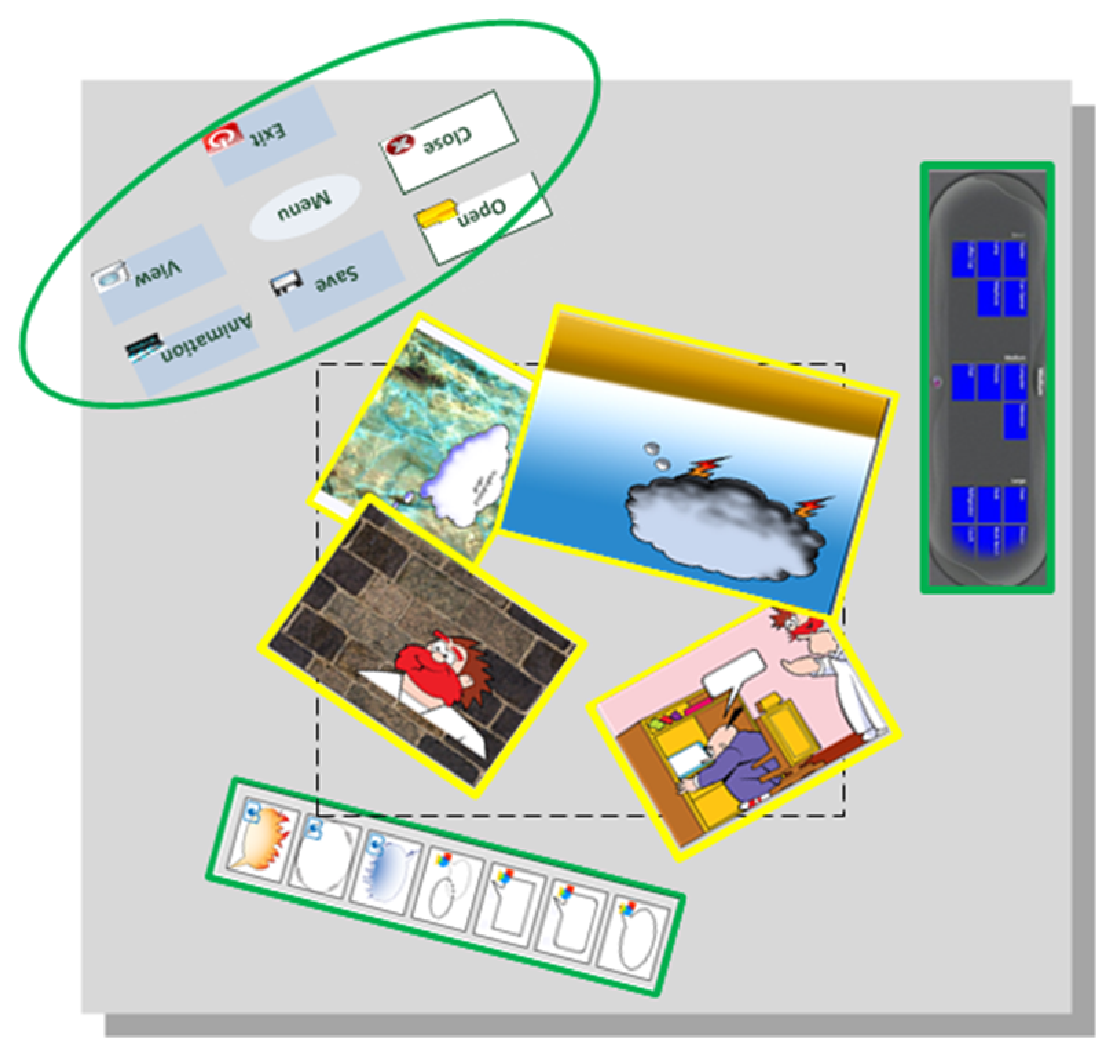
\includegraphics[scale=.3]{./img/applitable}
\caption{Application Table Interactive}
%\label{fig:applitable}
\end{figure}

 \end{columns}

\end{frame}

\begin{frame}[t]{Périmètres de la migration}
\setbeamercovered{transparent}
\textbf{{\small Hypothèses:}}
\begin{block}{{\small Application = interface utilisateur(UI) + noyau fonctionnel(NF)}}
{\scriptsize 	Considérons que le NF de l'application à migrer est réutilisé} \\
	 {\scriptsize $\Rightarrow$ Hétérogénéité des plateformes~\cite{TanenbaumS.1978}}\\
\end{block}
\pause
\textbf{{\small Pistes de migration d'UI:}}
\uncover<2>{
\begin{block}{{\small 1-Nouvelle conception de l'UI en prenant compte les principes de conception}}
	{\scriptsize \textbf{Coûts} de mise en \oe{}uvre}
\end{block}}
\pause
\uncover<3>{
\begin{block}{{\small 2-Déduire de l'UI à \textbf{partir du NF}{\tiny ~\cite{Kassoff2003}}}}
		%{\scriptsize  Comment choisir et placer les composants graphiques et les moyens d'\textbf{interactions} en se basant sur le NF?\\}
		{\scriptsize  Non Respect des \textbf{critères ergonomiques}}
\end{block}}
\pause
\uncover<4>{
\begin{block}{{\small 3-\textbf{Adapter} les éléments de l'UI de départ par rapport à la cible}}
	{\scriptsize Réutilisation et Respect des \textbf{critères ergonomiques}\\ }
	{\scriptsize $\Rightarrow$ Comment adapter la Structure, le Positionnement (Layout), le Style, les Interactions?}
%		\item {\scriptsize  Quels principes de conception d'UI pour de la plateforme cible?}
\end{block}
}
\end{frame}

\begin{frame}{Migration des UI sur des tables interactives }
\begin{figure}[t]
\centering
\includegraphics[scale=.3]{./img/aspectui}
%\caption{}
%\label{fig:aspectui}
\end{figure}
\begin{block}{Problèmes}
	\begin{itemize}
		\item {\small Quels principes de conception (guidelines) suivre pendant la migration?}\\
				{\tiny $\Rightarrow$ Quels types d'UI pour tables interactives? }
		\item {\small Comment adapter les différents aspects des UI à migrer?}\\
            {\tiny $\Rightarrow$ Quelles approches pour la migration d'UI?}

	\end{itemize}
\end{block}

\end{frame}

\section{Domaine d'étude }
\begin{frame}[t]{Tables interactives{\tiny ~\cite{MitsubishiElectricResearchLaboratoriesb, Ullmer1997, Microsoft2011}}}
\setbeamercovered{invisible}
\only<1>{
		\begin{figure}[t]
		\begin{center}
		\includegraphics[ scale=.35]{img/tablesinteractives}
		\end{center}
		\end{figure}}
\only<2>{
	{\scriptsize { Corpus de guidelines~\cite{Microsoft2011}}}
		\begin{figure}[t]
		\begin{center}
		\includegraphics[ scale=.4]{../chap2/img-23-1}
		\end{center}
		\end{figure}}
{\scriptsize$Type_{UI}=f(Utilisateurs, Instrument_{Interaction})$}\\
%\end{block}
		{\scriptsize {Utilisateurs (Nombre et Position) }}\\
%			\setbeamertemplate{itemize subitem}[circle]
%			\begin{itemize}
%				\item<2->  {\tiny Nombre d'utilisateurs}
%				\item<2->  {\tiny Répartition des utilisateurs}
%			\end{itemize}
		{\scriptsize {Instruments d'interactions=\{Dispositifs d'interactions, Bibliothèques Graphiques\} }}
%			\begin{itemize}
%				\item<2->  {\tiny Tangibilité des interactions}
%				\item<2->  {\tiny Tactibilité des interactions}
%%				\item<4->  {\tiny Taille de la surface d'affichage}
%%				\item<4->  {\tiny Disposition de la surface d'affichage}
%			\end{itemize}
	
\pause
\end{frame}

\section[État de l'art]{État de l'art des approches de migration}

\begin{frame}[t]{Caractéristiques des approches de migration d'UI}
\setbeamercovered{transparent}
$Approches Migration UI = \langle Source, Cible, M\acute ecanismes\rangle$
\pause
\begin{block}{Mécanismes }
\begin{itemize}
\item {\scriptsize Équivalences entre les instruments d'interactions}
\item {\scriptsize Adaptation des aspects de l'UI source} 
\item {\scriptsize Prise en comptes des guidelines}
\end{itemize}
{\tiny $\Rightarrow$ Ces mécanismes peuvent être manuels, automatiques ou semi automatiques}
\end{block}
\pause
\begin{block}{Evaluer chaque approche en tenant compte de }
\begin{itemize}
\item {\scriptsize la \textbf{flexibilité} des mécanismes ou du degrés d'intervention du concepteur pendant la migration, }
\item {\scriptsize la prise en compte des guidelines pour assurer une UI respectant les\textbf{ critères ergonomiques,}~\cite{Vanderdonckt1997}}
%\item {\scriptsize la  \textbf{généricité} ou l'indépendance des mécanismes par rapport aux applications ou plateformes, }
\item {\scriptsize la \textbf{réutilisabilité} du mécanisme d'adaptation ou d'équivalence qui est garantie par son indépendance par rapport aux applications ou plateformes}
\end{itemize}
\end{block}

%\begin{block}{{\small 1- \textbf{Équivalences} entre les éléments des plateformes source et cible}}
%{\scriptsize Comment se font les équivalences entre les instruments d'interactions ?	}
%		\begin{itemize}
%			\item {\tiny instruments d'interactions=bibliothèques graphiques + dispositifs d'interactions}
%		\end{itemize}
%%		\item {\tiny Comment les équivalences entre les modalités d'interactions sont établies? }
%\end{block}
%\pause
%\begin{block}{{\small 2- \textbf{Modélisation} des différents apects de l'UI}}
%{\scriptsize Est-ce que les mécanismes d'adaptation sont réutilisables?}
%	\begin{itemize}
%		 \item {\tiny Aspects UI=$ \{Structure,Layout ,Style, Interactions \}$}
%	\end{itemize}
%\end{block}
%\pause
%\begin{block}{{\small 3- Prise en compte des \textbf{Guidelines}}}
%{\scriptsize Comment les principes de conceptions d'UI pour la plateforme cible sont prises en compte ? }
%\begin{itemize}
%\item {\tiny basée sur les connaissances du concepteur} 
%\item {\tiny formalisée par des règles de transformations}
%\end{itemize}
%\end{block}

\end{frame}

\begin{frame}[t]{Migration de l'application AgilePlanner sur une table interactive{\tiny ~\cite{Wang2008}}}
\begin{itemize}
	\item {\scriptsize Approche ad hoc et manuelle de migration d'une UI}
	\item {\scriptsize Processus complet de migration en plusieurs étapes }
		\begin{enumerate}
			\item {\tiny Analyse}
			\item {\tiny Identification des guidelines}
			\item {\tiny Migration}
			\item {\tiny Évaluation}
		\end{enumerate}
\end{itemize}

\begin{figure}
\centering
\includegraphics[scale=.26]{./img/synthese1}
\end{figure}

%\begin{tabularx}{10cm}{|Y|Y|Y|}
%\hline {\scriptsize \textbf{Équivalences Manuelles}}  
%		\begin{itemize}
%          \item {\scriptsize des bibliothèques graphiques,}
%          \item {\scriptsize des dispositifs d’interactions}
%        \end{itemize}
%        &{\scriptsize \textbf{Guidelines} prises en compte par le concepteur en se basant sur ses connaissances} 
%        &{\scriptsize Aucun \textbf{Modèle} d'UI} \\ 
%\hline 
%\end{tabularx} 
{\scriptsize $\Rightarrow$ Mécanismes non réutilisables mais un résultat conforme aux attentes des utilisateurs finaux car flexibles}
\end{frame}

\begin{frame}[t]{Portage d'UI sur tables interactives{\tiny ~\cite{Besacier2010}}}
\begin{itemize}
\item {\scriptsize Migration sans re conception d'UI source}
\item {\scriptsize Approches spécifiques à des instruments d'interactions (Bibliothèques graphiques)}
%\item {\scriptsize Ensemble de techniques pour réutiliser les UI desktop sur des tables interactives}
%\item {\small Écriture des \textit{wrappers} entre bibliothèques graphiques}
%\item
\end{itemize}
\begin{figure}
\centering
\includegraphics[scale=.3]{./img/synthese2}
\end{figure}
{\scriptsize $\Rightarrow$  Mécanismes peu flexibles, réutilisables pour un ensemble  applications et produisant des UI peu utilisables}\\


%\begin{tabularx}{10cm}{|Y|Y|Y|}
%\hline {\scriptsize\textbf{Équivalences statiques} des bibliothèques graphiques}
%  & {\scriptsize \textbf{Guidelines} prises en compte partielles si la bibliothèque graphique cible est utilisée} 
%  & {\scriptsize Méta données pour caractériser Structure et les données} \\ 
%\hline 
%\end{tabularx} 

\end{frame}

\begin{frame}[t]{Services de migration d'UI{\tiny ~\cite{Paterno'2009}}}

\begin{block}{{\scriptsize  CRF~\cite{Calvary2002}: Modèles pour la conception d'UI multi plateformes}}
\begin{itemize}
\item {\tiny Tâches et concepts, AUI, CUI, FUI}
\item {\tiny Implémentations: USIXML, MARIAXML}
\end{itemize}
\end{block}
\only<1>{
\begin{block}{{\scriptsize Mécanismes de migration automatique d'UI}}

\begin{tabularx}{12cm}{Y Y}
\begin{flushleft}{\scriptsize Basés sur des modèles de conception} \newline  $\Rightarrow $ 
{\tiny Modèles de l'UI source sont fournies avec l'application à migrer}
\end{flushleft}
   &
   \begin{flushleft}{\scriptsize Basés sur une activité de Reverse Engineering(RE)} \newline
    $\Rightarrow $ {\tiny Modèles partiels de l'UI source sont retrouvés à partir de l'application à migrer } 
   \end{flushleft} \\ 

\end{tabularx} 
\end{block}
}
\only<2>{
\begin{figure}
\centering
\includegraphics[scale=.3]{./img/synthese3}
\end{figure}
{\scriptsize $\Rightarrow$  Mécanismes réutilisables et génériques pour des plateformes et des applications mais produisant des UI peu conformes aux critères ergonomiques car moins flexibles}}
\end{frame}

\begin{frame}[t]{MORPH{\tiny ~\cite{Moore1997} }}
\textit{Model Oriented Reengineering Process for HCI}
\only<1>{
\begin{itemize}
	\item {\scriptsize Processus de migration en trois phases}
			\begin{enumerate}
					\item {\tiny Détection}
					\item {\tiny Transformation}
					\item {\tiny Génération}
			\end{enumerate}
	\item {\scriptsize Approche basée sur des modèles abstraits (Structure, Tâches d'interactions)  }
		\begin{itemize}
				\item {\tiny Ajout manuel du layout et du style à l'UI migrée}
			\end{itemize}
%	\item {\scriptsize Modèles de tâches d'interactions non exhaustifs }
	\item {\scriptsize Mécanismes de prise en compte des guidelines peuvent être incorporés dans la base de connaissances}
	\item{\scriptsize Équivalences dynamiques basées sur un modèle de connaissances} 
	
\end{itemize}
}
\only<2>{
\begin{figure}
\centering
\includegraphics[scale=.3]{./img/synthese4}
\end{figure}
{\scriptsize $\Rightarrow$ Processus  réutilisable, produisant des UI conformes aux critères ergonomiques et plus flexible que les services de migrations d'UI mais n'offrant pas une assistance aux concepteurs }\\
 }
   
   

%\begin{tabularx}{10cm}{|Y|Y|Y|}
%\hline {\scriptsize \textbf{Équivalences Dynamique} des bibliothèques graphiques } 
%&{\scriptsize Prise en compte des \textbf{guidelines} dans la phase de transformation} 
%&{\scriptsize \textbf{Modèles} de tâches d'interactions, de Structure et Un modèle de connaissances} \\ 
%\hline 
%\end{tabularx} 

\end{frame}

\begin{frame}[t]{Synthèse}
\setbeamercovered{transparent}
%\begin{tabularx}{11cm}{|Y|Y|Y|Y|}
%\hline  	& {\small \textbf{Équivalences}} & {\small \textbf{Guidelines}} & {\small \textbf{ Modèles d'UI}}\\ 
%\hline {\tiny Migration Manuelle} 
%					& {\tiny Statique et non réutilisable}
%					& {\tiny Intuition}
%					& {\tiny Aucune Modélisation } \\ 
%\hline {\tiny Ré écriture de la boîte à outil} 
%					& {\tiny  Statique et réutilisable pour les même Boîte à outils}
%					& {\tiny Prise en compte partielle}
%					& {\tiny Aucune Modélisation} \\ 
%\hline {\tiny Migrations basées sur les modèles d'interactions et de structure} 
%					& {\tiny Dynamique}
%					& {\tiny Règles de transformation}
%					& {\tiny Interactions, Structure} \\ 
%\hline {\tiny Migration basées sur les Modèles CRF} 
%					& {\tiny Statique: Tables d'équivalences}
%					& {\tiny Règles de transformations}
%					& {\tiny Structure, Layout, Comportement, Interactions}\\ 
%\hline 
%\end{tabularx} 
%\begin{tabularx}{11cm}{|Y|Y|Y|}
%	\hline &+&-\\
%	\hline {\tiny \textbf{Équivalences}}& {\tiny - Les équivalences entre bibliothèque graphiques peuvent se faire à la volée si les éléments sont caractérisée avec un modèle de connaissances}
%	\newline {\tiny - Les équivalences entre les dispositifs d'interactions sont exprimée par les équivalences de bibliothèques graphiques}
%	& \\
%	\hline 
%\end{tabularx} 
%\begin{block}{{\scriptsize Approches de migrations}}
%	\begin{itemize}
%		\item<1-> {\scriptsize Les approches ad hoc produisent des UI conformes aux critères ergonomiques}
%%					\begin{itemize}
%%						\item {\tiny Les mécanismes de migrations sont adaptés à une application précise}
%%					\end{itemize}
%		\item<2-> {\scriptsize  La prise en compte des guidelines implique une transformation d'au moins un aspect de l'UI source}
%		% ou la non réutilisation de la structure et du layout  de l'UI source}
%		\item<3->  {\scriptsize Les approches semi automatiques sont flexibles et réduisent la tâche du concepteur}
%	\end{itemize}
%\end{block}
%\begin{block}{{\scriptsize Modèles d'UI}}
%\begin{itemize}
%\item<4-> {\scriptsize Les mécanismes de transformations  des aspects d'UI basées sur des modèles sont réutilisables}
%\item<5-> {\scriptsize Les modèles d'UI abstraits dans des approches RE doivent être exhaustifs et indépendants des domaines d'applications  }
%\end{itemize}
%\end{block}
%\begin{block}{{\scriptsize Équivalences des instruments d'interactions}}
%
%\begin{itemize}
%\item<6-> {\scriptsize Les équivalences dynamiques sont flexibles et facilitent la tâches du concepteur}
%
%\end{itemize}
%\end{block}
\begin{figure}[t]
\centering
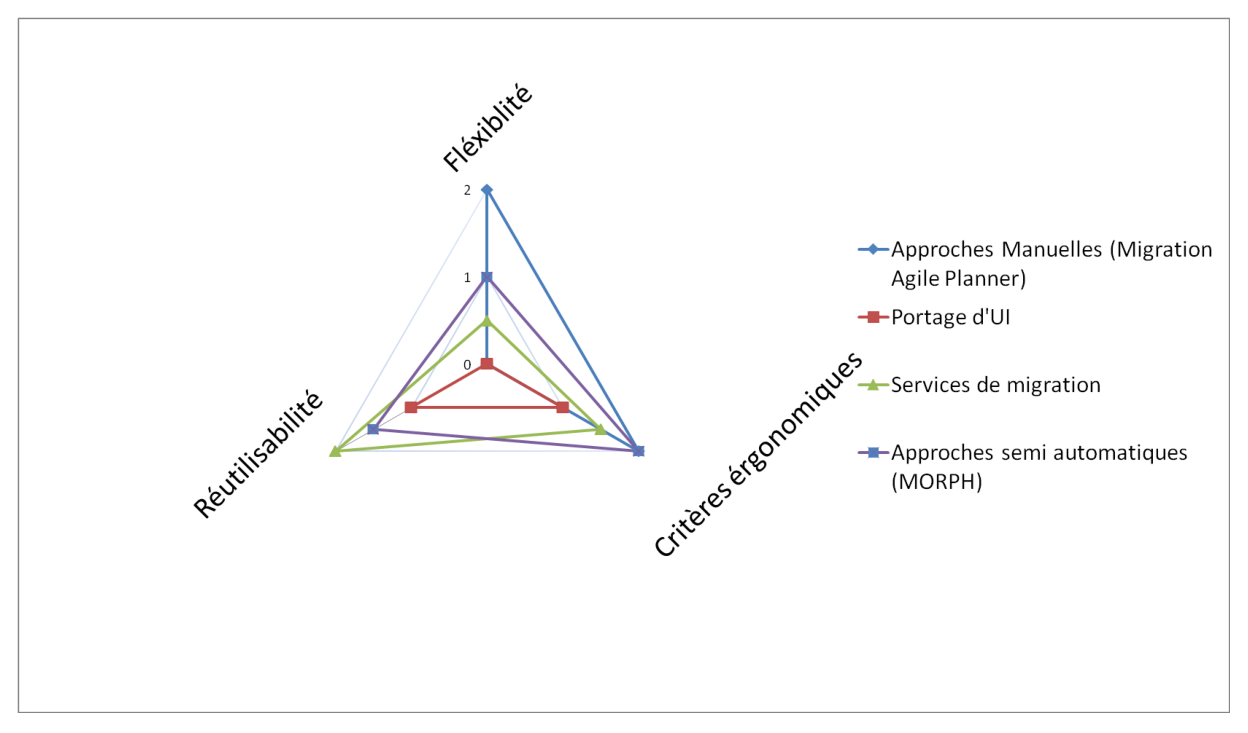
\includegraphics[scale=.5]{./img/syntheseapproches}
\caption{Synthèse des approches de migration d'UI}
\label{fig:syntheseapproches}
\end{figure}

\end{frame}

\begin{frame}[t]{Objectifs et Moyens}
\setbeamercovered{transparent}
\begin{block}{ {\small Migration des UI vers les tables interactives en respectant les critères ergonomiques de la cible}}
%\item {\small Ré engineering  des applications respectant une architecture }
\begin{itemize}
	\item {\tiny Mécanismes de reverse engineering d'UI (réutilisables)}
	\item {\tiny Mécanismes d'aide à la migration d'UI plus flexible à moindre \textbf{coût}}
\end{itemize}
\end{block}

\pause
\begin{block}{{\small Modélisation}}
{\tiny Proposer un modèle d'interactions abstraites qui permet}
\begin{itemize}
	\item {\tiny la \textbf{fléxibilité} de la prise en compte des guidelines pour décrire les équivalences}
\end{itemize}
\end{block}
\begin{block}{{\small Mécanismes de migrations d'UI vers les tables interactives}}
	\begin{itemize}
		\item {\tiny prise en compte des guidelines pendant la migration pour le respect des \textbf{critères ergonomiques} }
		\item {\tiny formalisation de la prise en compte des guidelines pour plus de \textbf{réutilisabilité}}
%		\item {\tiny l'assistance des concepteurs pendant les mécanismes de migration d'UI  }
%		\item {\tiny une prise en compte de toutes les guidelines identifiées}
	\end{itemize}
\end{block}

\end{frame}

\section{Modélisations}
\begin{frame}[t]{Interactions}
\setbeamercovered{transparent}
\only<1>{
\begin{block}{ { Interactions}}
\begin{figure}[t]
\begin{center}
\includegraphics[scale=.5]{../chap2/img-1}
\end{center}
\end{figure}
{\small $\Rightarrow$ Exprimer les actions, les commandes, les réponses et les feedback de l'UI par des interactions atomiques sur les \textbf{composants graphiques} : \textbf{Primitives d'interactions}}
\end{block}
}
\pause
\only<2-4>{
\begin{block}{{\small Primitives d'interactions}}
{\small $ComposantGraphique=\langle Propri\acute{e}t\acute{e}s\ graphiques,\ Contenu(s),\ Lien\ avec\ NF \rangle $}

\begin{columns}[t]
\begin{column}{.4\textwidth}
	{\small Propriétés graphiques } %(Taille, Position)} 
	\begin{itemize}
	\item {\scriptsize Widget Move} \item {\scriptsize Widget Rotation } \item {\scriptsize Widget Resize} \item {\scriptsize Widget Selection, Navigation}
	\item {\scriptsize Widget Display}
	\end{itemize}
\end{column}
\pause
\begin{column}{.33\textwidth}
	{\small Contenu(s)} 
	\begin{itemize}
	\item {\scriptsize Data Edition} \item {\scriptsize Data Selection} \item {\scriptsize Data Move In} \item {\scriptsize Data Move Out } 
	\item {\scriptsize Data Display}
	\end{itemize}

\end{column}
\pause
\begin{column}{.33\textwidth}
{\small Lien avec le NF}
	\begin{itemize}
		\item {\scriptsize  Activation}
	\end{itemize}
\end{column}

\end{columns}
\end{block}}

\end{frame}

\begin{frame}[t]{Primitives d'interactions et Composants graphiques}
\setbeamercovered{transparent}
% Modèles d'UI = Primitives d'interactions + Modèle de structure\\
 
	\begin{figure}[h]
	\includegraphics[ scale=.1]{../chap5/modelsutilises-2}
	\caption{\tiny {Modèles abstraits d'UI et UI finales}}
	\end{figure}
\pause
{\small Primitives d'interactions Intrinsèques}\\
{\small Primitives d'interactions Effective}
%	\begin{block}{{\small Primitives d'interactions Intrinsèques}}
%{\tiny 	Interactions atomiques \textbf{définies} des composants graphiques.\\} %
%	\end{block}
%	\begin{block}{{\small Primitives d'interactions Effective}}
%{\tiny 	Interactions atomiques des \textbf{instance} de composants graphiques.\\
%		Interactions réellement utilisées}	
%	\end{block}
\end{frame}

\begin{frame}[t]{Exemple de Primitives d'interactions}
\setbeamercovered{transparent}
\begin{columns}
	\begin{column}{0.3\textwidth}
	\begin{figure}[h]
	\begin{center}
	\includegraphics[scale=.3]{../chap4/img-1}
	%\caption{{\tiny Artéfact d'UI}}
	\end{center}
	\end{figure}
	\end{column}
	\begin{column}{.8\textwidth}
	\begin{table}[t]
	\begin{tabularx}{8cm}{|Y|Y|}
	\hline  \textbf{{\tiny Composants graphiques}} & \textbf{{\tiny Primitives d'interactions} }\\ 
	\hline {\tiny Liste d'images} & 
			{\tiny 	Widget Selection, Navigation, Widget Display, Data Selection,  Data Move Out, Activation  \newline Data Display }\\ 
	\hline {\tiny Liste déroulante }& 
				{\tiny Widget Selection, Navigation, Data Selection, Data Display, Activation} \\ 
	\hline 
	
	\end{tabularx} 
	%\caption{{\tiny Exemple de primitives d'interactions}}
	\end{table}
	
	\end{column}
\end{columns}
\pause
%	\begin{block}{{\small Remarques} }
	\begin{itemize}
		\item {\scriptsize Les \textbf{primitives d'interactions} permettent de décrire les interactions entre UI et l'utilisateur \textbf{indépendamment des instruments d'interactions} }
		\item {\scriptsize Comment décrire les \textbf{équivalences des composants graphiques} avec les primitives d'interactions?} 
	\end{itemize}
%	\end{block}
\end{frame}

\begin{frame}[t]{Équivalences des composants graphiques}
\setbeamercovered{transparent}
{\scriptsize $Composant Graphique=\langle Cardinalit\acute e, TypeDeDonn\acute ee , PrimitivesInteractions\rangle$}

\begin{block}{{\scriptsize Opérateurs d'équivalences basés sur des PI(Primitives d'Interactions) }}
\begin{columns}
	\begin{column}{.4\textwidth}
\begin{itemize}
\item<1> $ \equiv ${\tiny Équivalence stricte des PI}
\item<2> $ \leqq ${\tiny Équivalence large des PI} 
\item<3> $\geqq ${\tiny Équivalence faible des PI} 
\end{itemize}
\end{column}
	
\begin{column}{.7\textwidth}
	\begin{center}
	%{\scriptsize $Source\ operateur\ Cible$ }
	\only<1>{
{\tiny JButton $\equiv$ SurfaceButton\\
$\left\lbrace \begin{array}{c}
Navigation\\ Widget Selection\\ Activation
\end{array} \right \rbrace \equiv 
\left\lbrace \begin{array}{c}
Navigation\\ Widget Selection\\ Activation
\end{array} \right\rbrace $}}
\only<2>{
{\tiny JFrame $\cong $ DSFrame \\
$\left\lbrace \begin{array}{c}
Navigation\\ Widget Selection\\ Widget Display\\ Widget Move\\ Widget Resize\\ Activation
\end{array} \right \rbrace
 \leqq
\left\lbrace \begin{array}{c}
Navigation\\ Widget Selection\\  Widget Display\\ Widget Move\\ Widget Resize\\ Activation\\ \color{red}{WidgetRotation}
\end{array} \right\rbrace $}}
	\only<3>{
{\tiny ListBox (Éditable) $ \geqq $ SurfaceTextBox \\
$\left\lbrace \begin{array}{c}
Navigation\\ Widget Selection\\ Widget Display\\Data Edition\\ \color{red}{ Data Selection}\\ Activation
\end{array} \right \rbrace
\geqq
\left\lbrace \begin{array}{c}
Navigation\\ Widget Selection\\ Widget Display\\ Data Edition\\ Activation
\end{array} \right\rbrace $}
	}
	\end{center}
	\end{column}
\end{columns}
\pause[4]
\end{block}
\begin{block}{{\scriptsize Opérateurs d'équivalences basés sur des PI et les types de données }}
\begin{columns}
	\begin{column}{.4\textwidth}
\begin{itemize}
\item<4> $ \cong ${\tiny Équivalence stricte des PI et type de données différentes}
\item<5>  $ \lesssim ${\tiny Équivalence large des PI  et type de données différentes}
\item<6>  $ \gtrsim ${\tiny Équivalence faible des PI  et type de données différentes}
\end{itemize}
\end{column}
	
\begin{column}{.7\textwidth}
\begin{center}
\only<4>{
	{\tiny ListBox $\approxeq $ LibraryBar \\
	$\left\lbrace \begin{array}{c}
	Navigation\\ Widget Selection\\ Widget Display\\ DataSelection[t1]\\ DataMove In/Out[t1]\\ DataDisplay[t1]\\ Activation
	\end{array} \right \rbrace
	 \cong 
	\left\lbrace \begin{array}{c}
	Navigation\\ Widget Selection\\ Widget Display\\ \color{green}{DataSelection[t2]}\\ \color{green}{DataMove In/Out[t2]}\\ \color{green}{DataDisplay[t2]}\\ Activation
	\end{array} \right\rbrace $\\ $t1=String, t2=MediaElement$ }
}
\only<5>{
	{\tiny Button $\lesssim $ Image \\
	$\left\lbrace \begin{array}{c}
	Navigation\\ Widget Selection\\ Widget Display\\ Activation
	\end{array} \right \rbrace
	 \lesssim 
	\left\lbrace \begin{array}{c}
	Navigation\\ Widget Selection\\ Widget Display\\ \color{green}{DataDisplay[t]}\\ Activation
	\end{array} \right\rbrace $\\ $ t=MediaElement$ }
}
\only<6>{
	{\tiny Image $\gtrsim$ SurfaceButton  \\
	$\left\lbrace \begin{array}{c}
	Navigation\\ Widget Selection\\ Widget Display\\ \color{green}{DataDisplay[t]}\\ Activation
	\end{array} \right \rbrace
	 \gtrsim
	\left\lbrace \begin{array}{c}
	Navigation\\ Widget Selection\\ Widget Display\\ Activation
	\end{array} \right\rbrace $\\ $ t=MediaElement$ }
}

\end{center}
\end{column}
\end{columns}
\end{block}
\end{frame}

\begin{frame}[t]{Exemple d'équivalences}{\scriptsize $Source=XAML\  et\ Cible=XAMLSurface$}
\setbeamercovered{transparent}
\begin{columns}
	\begin{column}{.25\textwidth}
	\begin{figure}[t]
	\centering
	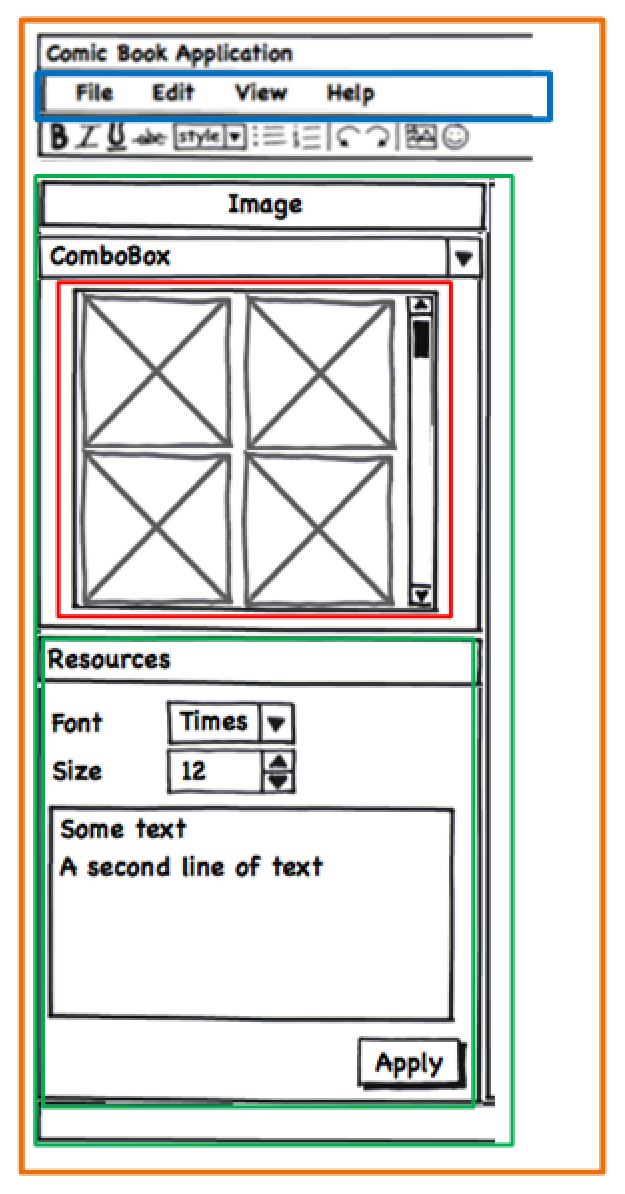
\includegraphics[scale=.27]{img/exempleequiv}
	\end{figure}
	\end{column}
	\begin{column}{.82\textwidth}
	\begin{table}[t]
		\begin{tabularx}{9cm}{|Y|Y|Y|Y|}
			\hline & $\equiv/\approxeq$ &  $  \leqq/ \lesssim $ & $ \geqq/\gtrsim$ \\
			\hline \textcolor{orange}{{\tiny Window }}&-/- &-/- & {\tiny SurfaceWindow}{\tiny /-} \\
%			\hline \textcolor{blue}{{\tiny Menu}}
%			& {\tiny ElementMenu, SurfaceMenu } /
%			& {\tiny SurfaceListBox}{\tiny / LibraryBar}
%			& \\
%			\hline \textcolor{green}{{\tiny Grid}}
%			&{\tiny  Grid}/-
%			&{\tiny ScatterView}/- & \\
			\hline \textcolor{red}{{\tiny ListBox}}
			& {\tiny SurfaceListBox / LibraryBar}
			& -/-
			& {\tiny ElementMenu, SurfaceMenu / DataGrid}\\
			\hline
		\end{tabularx}
	\end{table}
	\pause
%	\begin{block}{{\scriptsize Remarques}}
	\begin{itemize}
%		\item{\scriptsize Les 6 opérateurs permettent d'établir des \textbf{équivalences }}
		\item {\scriptsize Quels composants graphiques \textbf{sélectionner} si plusieurs correspondants?} 
		\item {\scriptsize Comment \textbf{transformer} l'UI source en prenant en compte les guidelines?}
	\end{itemize}
%	\end{block}
	\end{column}
\end{columns}
\end{frame}

\begin{frame}[t]{ Transformations de la structure d'UI source}
\setbeamercovered{invisible}
{\scriptsize UI cible obtenue en remplaçant les éléments de la source}
\begin{block}{{\scriptsize  Substitution 1$ \rightarrow$ 1}}
\begin{itemize}
\item{\tiny Remplacer un élément de l'UI source par son \textbf{équivalent} sur la cible (conformément aux opérateurs d'équivalences)}
\item {\tiny Exemple(JavaSwing vers DiamondTouch): JFrame correspond à DSFrame}
\end{itemize}
\end{block}
\pause
\begin{block}{{\scriptsize Substitution n $ \rightarrow$ m } {\tiny avec $ n\geq 1, m\geq 1$ }}
{\tiny Remplacer un \textbf{groupe} d'éléments d'UI par un ou plusieurs élément(s) équivalent\\}
{\tiny $\Rightarrow$ Comment choisir les groupes ?}
\end{block}

\begin{block}{{\scriptsize Exemples}}
\begin{columns}
\begin{column}{.3\textwidth}
\only<2>{{\tiny  Substitution 4 à 4 en appliquant la guideline d'UI collaborative}}
\only<4> {{\tiny Substitution 2 à 1 }}
\only<3> {{\tiny Substitution 1 à 2 en appliquant la guideline d'UI Tangible}}
\end{column}
\begin{column}{.7\textwidth} \only<2>{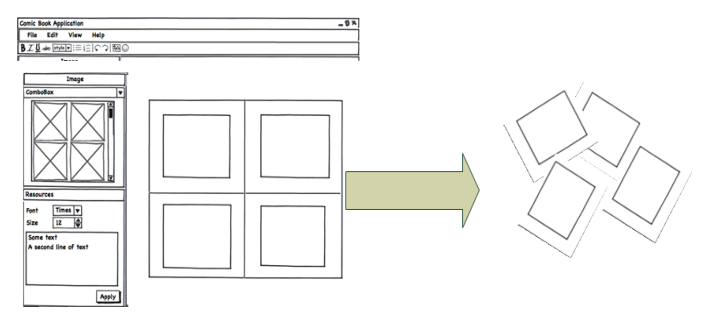
\includegraphics[scale=.4]{./img/transfo1to4}} 
\only<4>{\includegraphics[scale=.4]{./img/transfo2to1}} 
\only<3>{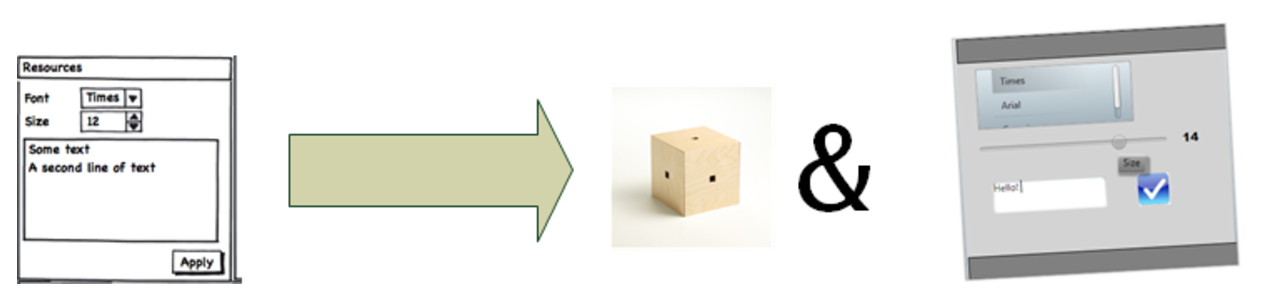
\includegraphics[scale=.3]{./img/transfo1to2}}
% &   \\ 
%{ %\tiny  Équivalence 4 à 4 en appliquant la guideline d'UI collaborative }& {\tiny Équivalence 2 à 1}\\
\end{column}
\end{columns} 

\end{block}
\end{frame}

\begin{frame}[t]{Modèle de structure}
\setbeamercovered{transparent}
 %Contenance + Type de données + Cardinalité +Primitives d'interactions effectives}
\begin{block}{{\scriptsize Exprime une instance d'UI}}
\begin{itemize}
\item {\scriptsize Primitives d'interactions effectives}
\item {\scriptsize \textbf{Données} des composants graphiques (Type de données, Cardinalité)}
\item {\scriptsize Liens de contenance entre composants graphiques: Pour exprimer les \textbf{groupes}}
\begin{itemize}
	\item{\tiny  \textbf{UIComponent}: élément d'UI simple}
	\item {\tiny \textbf{Container}: élément d'UI  contenant d'autres, exprime un \textbf{groupe} d'élément d'UI}
\end{itemize}
\end{itemize}
\pause   

\begin{table}[t]
\begin{tabularx}{10cm}{|Y|Y|}
\hline  {\tiny Contenu} & {\tiny Type de container} \\
\hline{\tiny  $\{UIComponent\}$} & 
{\tiny \textbf{Homogène}: données du même type \newline \textbf{Hétérogène}: données de types différents }\\ 
\hline {\tiny $\{ UIComponent\}\cup \{Container\} $} &
{\tiny \textbf{Hétérogène:} si a un parent} \\ 
\hline{\tiny  $ \{Container\} $ }&{\tiny \textbf{Récursif:} si contient des containers} \\ 
\hline 
\end{tabularx} 
\end{table}
%\begin{tabular}{cccc}
%{\tiny \textbf{Window}}& {\tiny \textbf{Simple}}&  {\tiny \textbf{Panel}}& {\tiny \textbf{Table}} \\ 
%\end{tabular}
{\scriptsize Type Container= \textbf{Racine}  si pas de parent}
 
\end{block}

\end{frame}

\begin{frame}[t]{Exemple Modèle de structure } %Prise en compte des Guidelines}
\setbeamercovered{transparent}
% TODO:
%Dire comment les Guidelines sont prise en compte pendant la transformation de la structure et la sélections
\begin{figure}[t]
\includegraphics[scale=.35]{../chap4/typecontainers}
%\caption{{\tiny Illustration des types de container}}
%\label{fig:chap4:5}
\end{figure}
{\scriptsize $ \Rightarrow Mod\grave ele UI = Mod\grave ele\ de\ Structure + Primitives\ Interactions $}
\pause
\begin{block}{{\scriptsize \textbf{Transformations} du modèle d'UI en prenant en compte les \textbf{guidelines} }}
%\begin{itemize}
%\item {\scriptsize UI Collaborative}
%	\begin{itemize}
%	\item {\tiny Menus utilisables par tous les utilisateurs} 
%	\item {\tiny Formulaires, Tableaux, Zones de contenus accessibles}
%	\end{itemize}
%\item {\scriptsize UI Tangible: Utiliser des objets tangibles}
%	\begin{itemize}
%		\item {\tiny pour afficher un groupe de composants graphiques (formulaires, tableaux, panels, menus)}
%		\item {\tiny pour activer des fonctionnalités}
%	\end{itemize}
%\end{itemize}
\end{block}

\end{frame}

\begin{frame}{Rappel des guidelines}
	{\scriptsize { Corpus de guidelines~\cite{Microsoft2011}}}
		\begin{figure}[t]
		\begin{center}
		\includegraphics[ scale=.4]{../chap2/img-23-1}
		\end{center}
		\end{figure}
\end{frame}
\section[Mécanismes]{Mécanismes de migrations}

\begin{frame}[t]{{\small Prise en compte des guidelines: Transformations} } %{Transformations de l'UI source}
\setbeamercovered{transparent}
\setbeamerfont{enumerate subsubbody}{size=\tiny	}
\begin{columns}
\begin{column}{.5\textwidth}
\begin{block}{{\tiny Règle 1: Container de type Récursif}}
%{\tiny $Simple=\{Container\}$}
%\begin{enumerate}
{\tiny Appliquer la guideline d'utilisation en 360 degrés de l'UI (UI Collaborative)  }
%\end{enumerate}
\end{block}
\pause
\begin{block}{{\tiny Règle 2: Container de type Homogène}}
%{\tiny $Table=\{UIComponent\}$ avec données du même type}
%\begin{enumerate}
{\tiny Appliquer les guidelines d'utilisation des Objets Tangibles (UI Tangible)  }
%\end{enumerate}
\end{block}
\pause
\end{column}

\begin{column}{.5\textwidth}
\begin{block}{{\tiny Règle 3: Container de type Hétérogène}}
%{\tiny $Panel=\{UIComponent\}$ }
%\begin{enumerate}
{\tiny Si parent est un Récursif alors cf. Règle 1}
%\end{enumerate}
\end{block}
\pause
\begin{block}{{\tiny Règle 4: Container de type Racine}}
%{\tiny $Window=Element Racine$}
%\begin{enumerate}
{\tiny Si tous les fils sont Container alors appliquer Règle 1\\}
{\tiny Sinon Appliquer la guideline de partage d'espace de travail (G6) en fonction du nombre d'utilisateurs (G4)}
%\end{enumerate}
\end{block}
\end{column}
\end{columns}
\begin{figure}[t]
\begin{center}
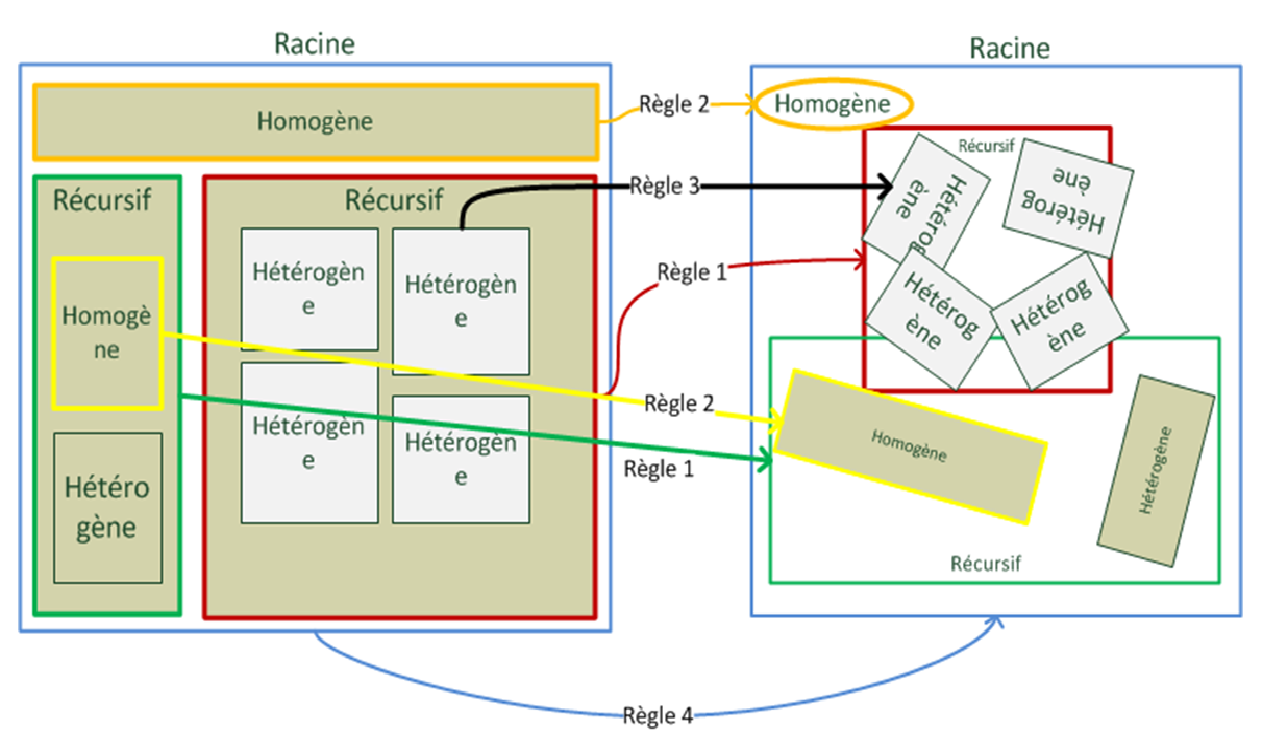
\includegraphics[scale=.27]{./img/transforule}
%\caption{Transformations}
\end{center}
\end{figure}

{\scriptsize $\Rightarrow\ Et\ la\ concr\acute{e}tisation\ du\ mod\grave{e}le\ transform\acute{e}!$}



\end{frame}
\begin{frame}[t]{{\small Prise en compte des guidelines:Sélection des composants graphiques }}
%{}
\setbeamercovered{invisible}
\begin{block}{{\scriptsize Plusieurs opérateurs d'équivalence!}}
	\begin{itemize}
		\item {\tiny Plusieurs composants graphiques cible équivalents}
		\item {\tiny Méthode de classement suivant les Utilisateurs finaux et le concepteur}
	\end{itemize}
\end{block}
\pause
\begin{block}{{\scriptsize Classement des composants graphiques équivalents}}
{\scriptsize Deux critères}
\begin{itemize}
	\item {\tiny Conformité aux guidelines }
	\item{\tiny  Coût de la mise en \oe{}uvre (Nouvelles ressources, Fonctionnalités supplémentaires, ...)}

\end{itemize}
 {\scriptsize Importance d'un composant graphique = Conformité aux guidelines - Coût de la mise en \oe{}uvre}
\end{block}
\begin{block}{{\scriptsize Exemple}}
\only<2>{
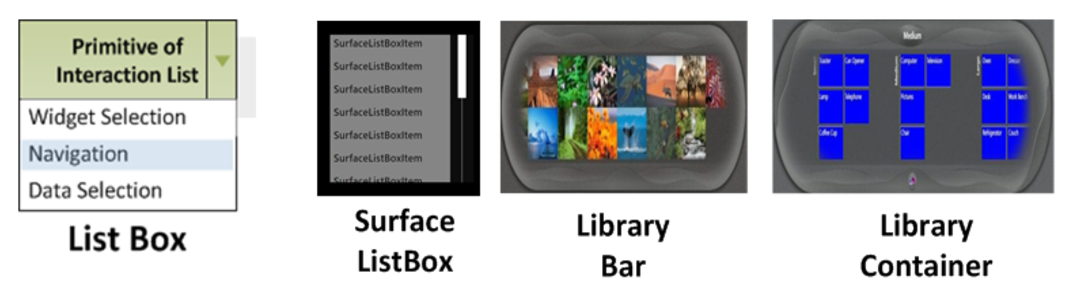
\includegraphics[scale=.3]{./img/selection}}
\only<3>{\includegraphics[scale=.3]{./img/exempleequiv1}}
\end{block}

\end{frame}


\section{Implémentation}

\begin{frame}{Migration assitée d'UI vers les tables interactions}
{Processus de migration}
\begin{figure}[t]
\begin{center}
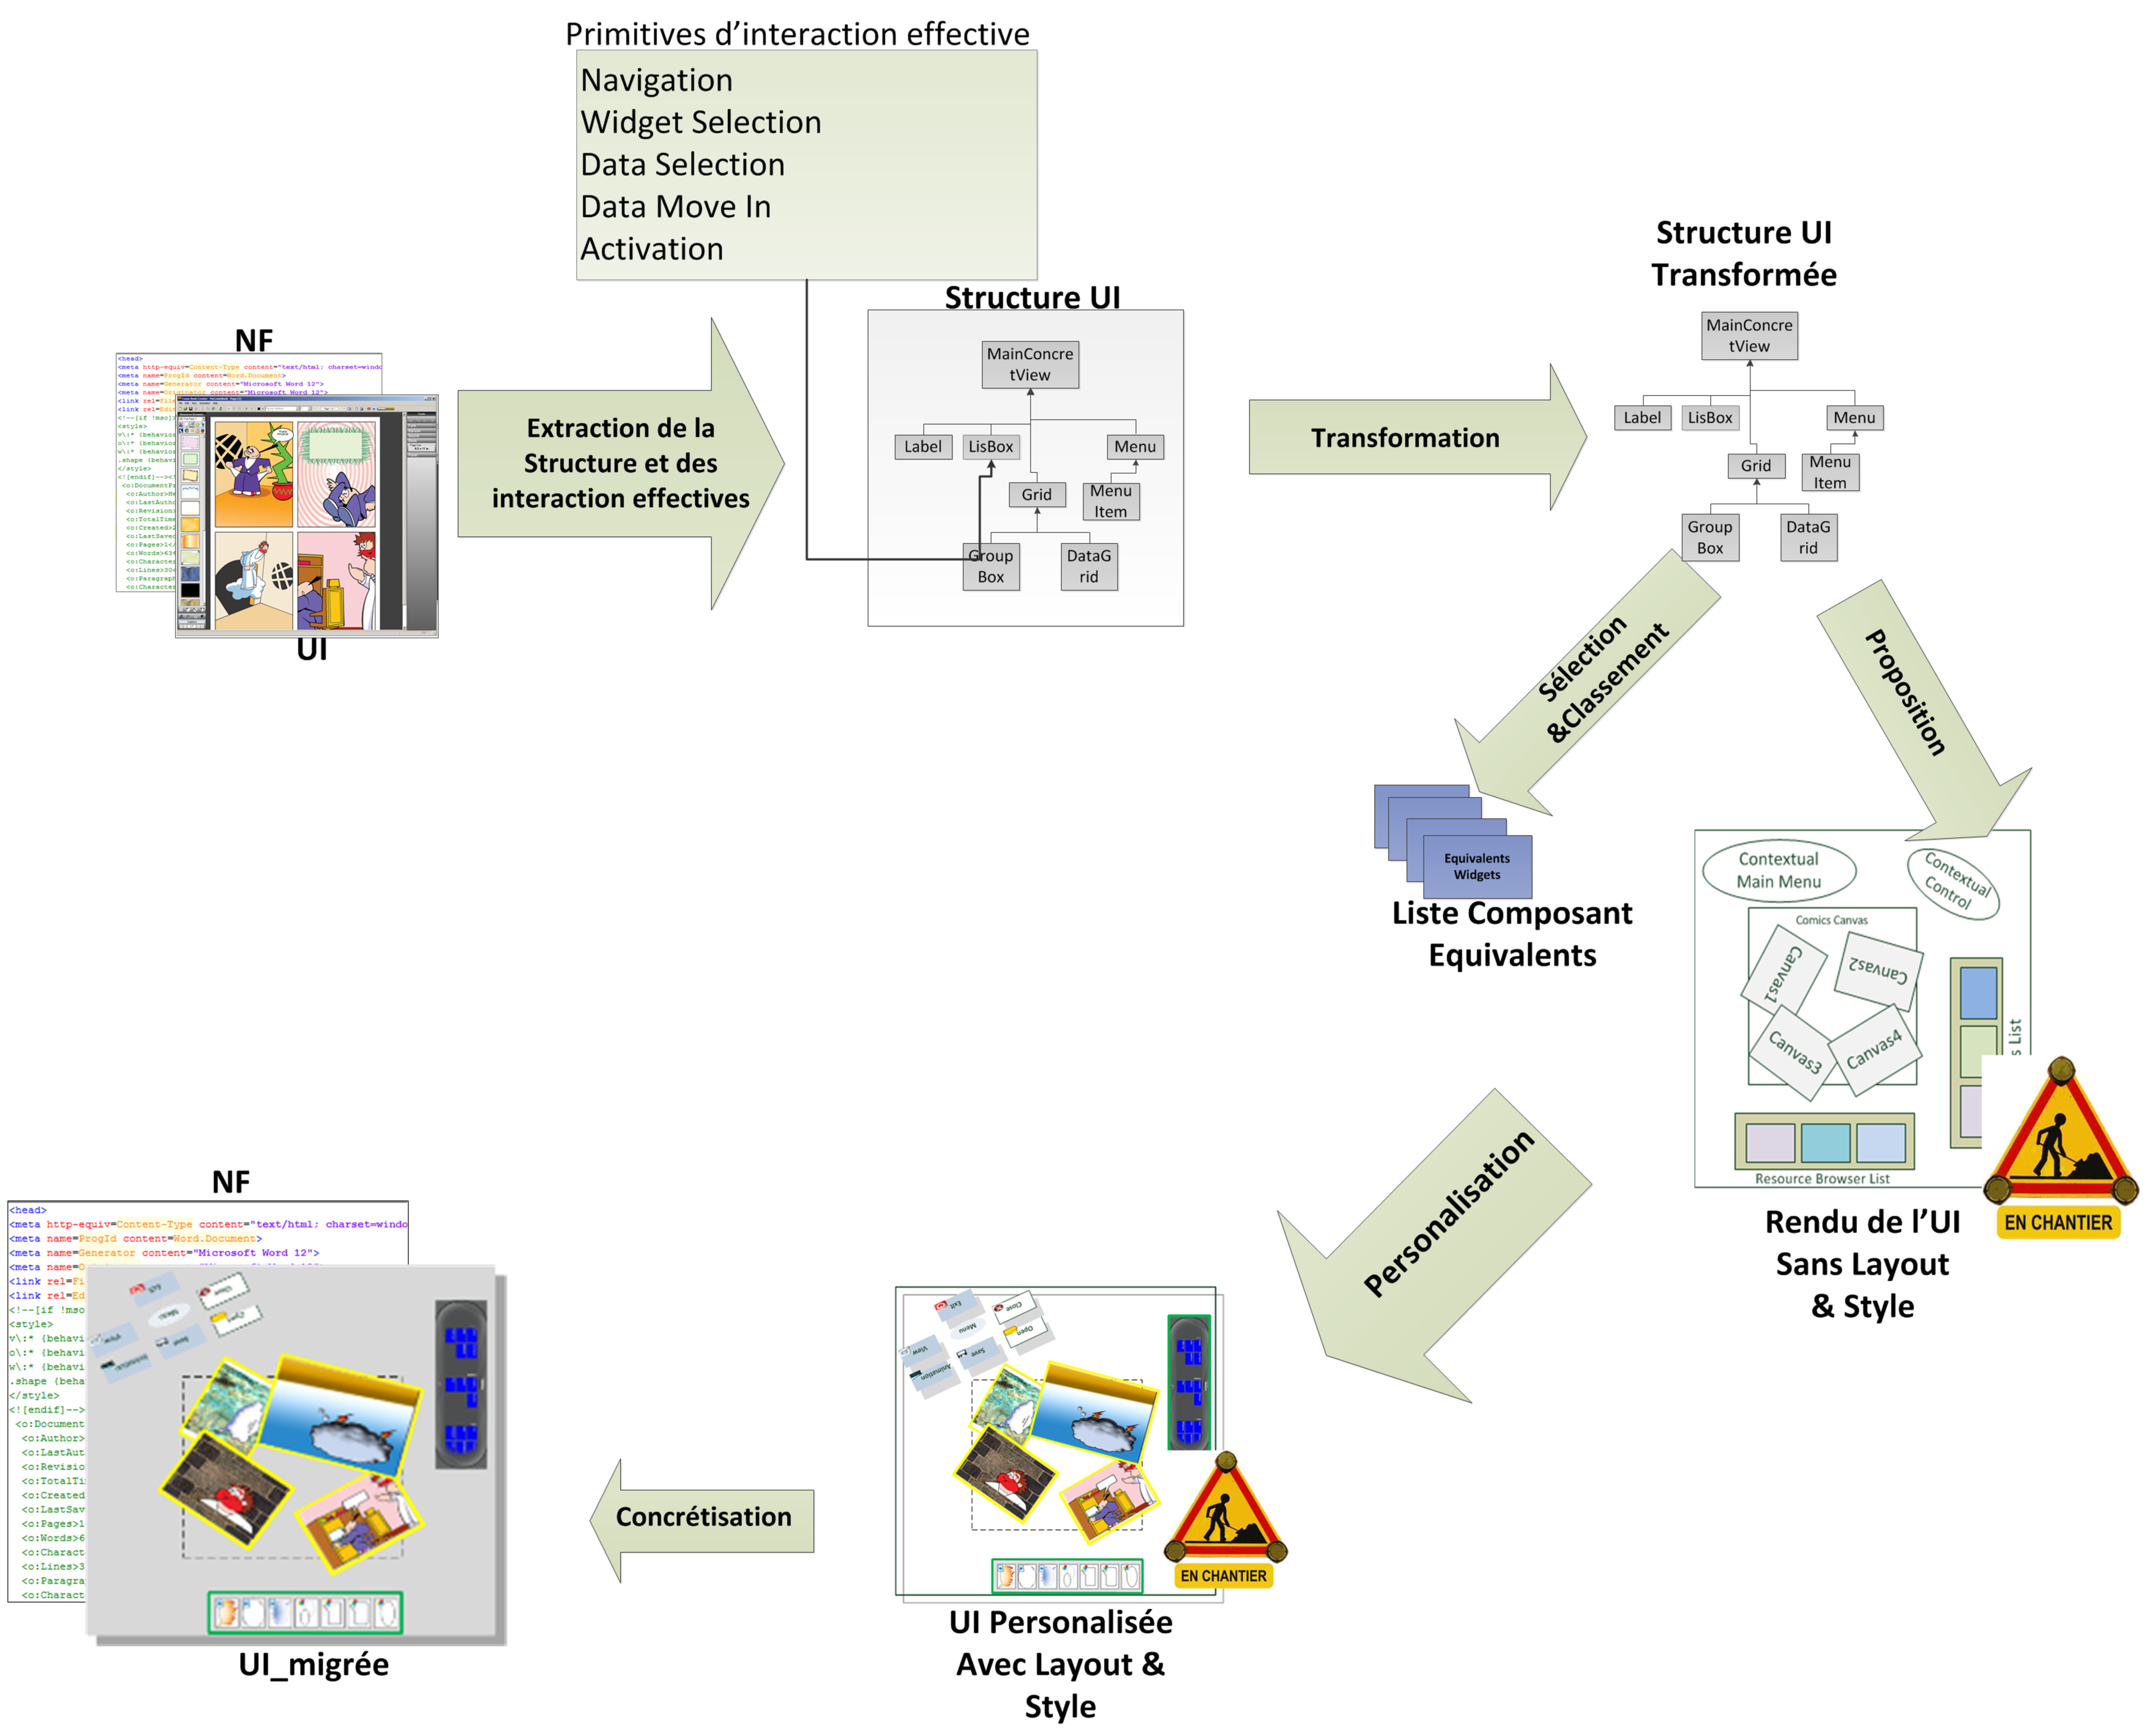
\includegraphics[scale=.12]{./img/process}

\end{center}\end{figure}

\end{frame}
\begin{frame}{Implémentations }
\begin{block}{Équivalences des composants graphiques à base des primitives d'interactions}
	\begin{itemize}
		\item Abstraction du modèle de structure et des primitives d'interactions d'une UI XAML 
		\item Équivalences et classement des composants graphiques
	\end{itemize}
\end{block}

\begin{block}{Editeur graphique pour table interactive}
\begin{itemize}
\item Outil d'affichage et de manipulation d'UI à partir d'une instance du modèle d'UI
\item Génération du fichier XAML pour Microsoft PixelSense
\end{itemize}
\end{block}


\end{frame}

\section[Conclusions]{Conclusions et perspectives}

\begin{frame}{Conclusions }
\begin{block}{{\small Conclusion de la thèse}}
\begin{itemize}
\item {\scriptsize Les \textbf{primitives d'interactions} permettent de décrire des mécanismes d'équivalences \textbf{réutilisables} et \textbf{flexibles} en prenant compte les guidelines}
\item {\scriptsize Les mécanismes de migrations basés sur le \textbf{modèle de structure} et les \textbf{primitives d'interactions} prennent en compte les guidelines spécifiques à la cible }
\end{itemize}
\end{block}
\pause
\begin{block}{Perspectives de cette thèse}
\begin{itemize}
\item {\scriptsize Extension des mécanismes de transformations de structure à d'autres plateformes }
\item {\scriptsize Plateforme d'aide à la migration réutilisable pour un ensemble de plateformes}
\end{itemize}
\end{block}
\end{frame}
\begin{frame}{État d'avancement de la rédaction}

\begin{block}{{\scriptsize État d'avancement de la rédaction}}
\begin{tabular}{|l|l|} 	
\hline {\tiny \textbf{Chapitres}}  &  {\tiny \textbf{État}} \\ 
\hline {\tiny 1-Tables interactives et Migration d'UI} 
					& {\tiny Terminé (Lu par Audrey(2) et Gaetan(1))} \\ 
\hline {\tiny 2-Approches de migration d'UI} 
					& {\tiny Terminé (Lu par Audrey(2))} \\ 
\hline {\tiny 3-Modélisation des interactions abstraites} 
					& {\tiny En cours (Lu par Audrey(1), Philippe(2))}  \\ 
\hline {\tiny 4-Prise en compte des guidelines} 
					&  {\tiny En cours (Lu par Audrey(1))}\\ 
\hline {\tiny 5-Prototype} 
					& {\tiny 70 \% fait} \\ 
\hline 
\end{tabular} 
\end{block}

\pause
\begin{block}{Rédactions Perspectives}
	\begin{itemize}
		\item Fin de la rédaction Début Janvier 
		\item Soutenance février ou début mars 2013
	\end{itemize}
\end{block}
\end{frame}

\begin{frame}{}
\begin{figure}
\centering
\includegraphics[scale=.5]{./img/questionimg}
%\caption{}
%\label{fig:questionimg}
\end{figure}

\end{frame}
\begin{frame}[allowframebreaks]{Bibliographie}
	\bibliographystyle{plainnat}
	\tiny
	\bibliography{../bib/biblio} 
\end{frame}

\begin{frame}{Detail 1: Extraction des primitives d'interactions}
\thispagestyle{empty}
%\setcounter{framenumber}{0}
\end{frame}
\begin{frame}{Detail 2: Opérateurs d'équivalences}
\thispagestyle{empty}
%\setcounter{framenumber}{0}
	\begin{table}[t]
		\begin{tabularx}{9cm}{|Y|Y|Y|Y|}
			\hline & $\equiv/\approxeq$ &  $  \leqq/ \lesssim $ & $ \geqq/\gtrsim$ \\
			\hline \textcolor{orange}{{\tiny Window }}&-/- &-/- & {\tiny SurfaceWindow}{\tiny /-} \\
			\hline \textcolor{blue}{{\tiny Menu}}
			& {\tiny ElementMenu, SurfaceMenu } /
			& {\tiny SurfaceListBox}{\tiny / LibraryBar}
			& \\
			\hline \textcolor{green}{{\tiny Grid}}
			&{\tiny  Grid}/-
			&{\tiny ScatterView}/- & \\
			\hline \textcolor{red}{{\tiny ListBox}}
			& {\tiny SurfaceListBox }/{\tiny LibraryBar}
			& -/-
			& \\
			\hline
		\end{tabularx}
	\end{table}

\end{frame}
\begin{frame}{Detail 3: Règles de transformations}
\thispagestyle{empty}
%\setcounter{framenumber}{0}
\begin{figure}
\centering
\includegraphics[scale=.4]{./img/selection1}
\end{figure}

\end{frame}
\begin{frame}{Detail 4: Guidelines}
\thispagestyle{empty}
%\setcounter{page}{0}
\begin{figure}
\centering
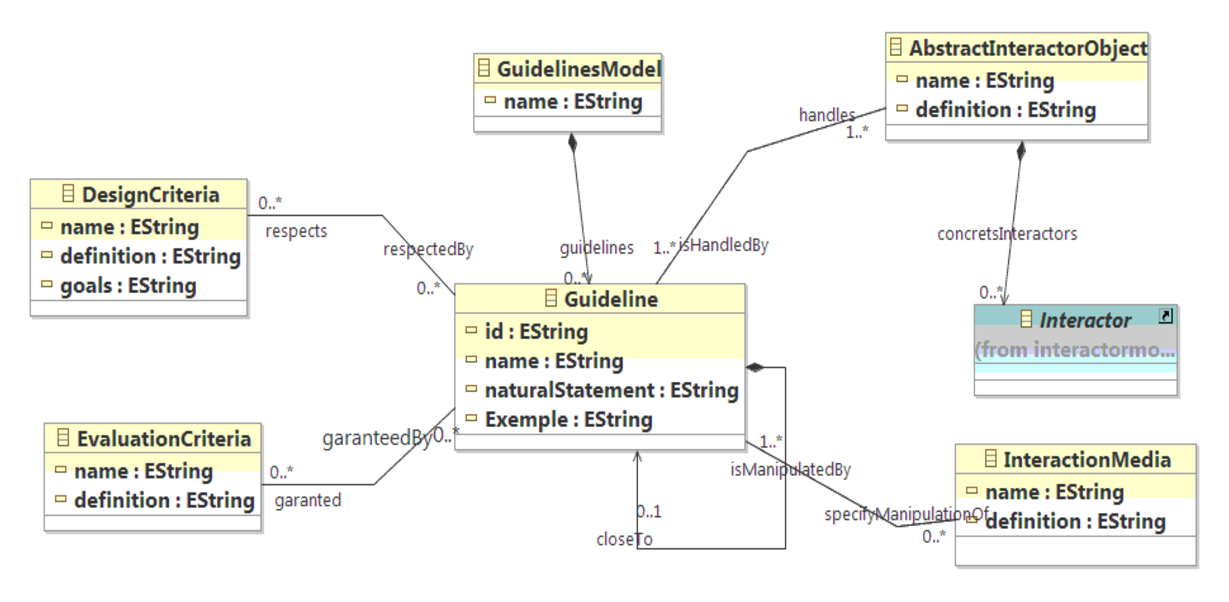
\includegraphics[scale=.5]{./img/guidelinesmodeles}
\caption{}
\label{fig:guidelinesmodèles}
\end{figure}

\end{frame}


\end{document}
